\chapter{Handicap et emploi}
\label{handicap_emploi}

Les personnes marquées par un handicap à la naissance ou un handicap acquis dans les suites d'un accident ou d'une maladie se retrouvent en situation de "surhandicap" quand elles sont confrontées à des difficultés d'insertion ou de réinsertion professionnelle. Pour introduire le sujet, il importe de préciser les supports conceptuels et les dispositifs législatifs qui entourent le handicap en rappelant quelques notions de base.

\section{Le Handicap : un processus "dynamique"}
Handicap est un mot simple qui tire son origine de l'expression "hand in the cap" (la main dans le chapeau). Cette expression désignait une transaction au cours de laquelle deux personnes, souhaitant échanger des objets de valeur différente, confiaient le r\^ole d'arbitre à un tiers. Ce dernier évaluait la somme d'argent à ajouter à l'objet de moindre valeur pour que l'échange soit équitable. La transaction se déroulait ensuite dans un chapeau dans lequel les participants plaçaient la somme qu'ils jugeaient adéquate.\\

Le mot Handicap est également appliqué à la compétition équestre. Lorsque deux chevaux de calibres différents concourraient ensemble, le meilleur était lesté d’un poids appelé « handicap » afin de maintenir l’égalité de chance entre les deux.\\
Cette étymologie a conservé son sens au point de sous-tendre, sans le dire explicitement la loi sur l'égalité des droits et des chances des personnes handicapées.\\

\noindent La loi cadre de février 2005 pour l'égalité des droits et des chances, la participation et la citoyenneté des personnes handicapées met à jour une approche évoluée du handicap :

\begin{quotation}
\noindent Constitue un handicap, au sens de la présente loi, toute limitation d’activité ou restriction de participation à la vie en société \underline{subie dans son environnement} par une personne en raison d’une altération substantielle, durable ou définitive d’une ou plusieurs fonctions physiques, sensorielles, mentales, cognitives ou psychiques, d’un polyhandicapé ou d’un trouble de santé invalidant.\\
\end{quotation}


Le schéma de Wood a longtemps prévalu (Figure \ref{schema_wood}). Il était fondé sur un schéma linéaire reliant à l'origine la \textbf{Déficience} (ex. une hémiplégie ou une paraplégie) à l'\textbf{Incapacité} (ex. incapacité de marcher ou de tenir un objet) puis au \textbf{Handicap} (désavantage social résultant des 2 concepts précédents: ex. ne pas pouvoir reprendre une activité professionnelle). Tout ceci était vu sous un angle linéaire comme s'il existait un continuum incontournable entre les 3 concepts. \\

Le modèle de Wood s'est avéré incomplet car certains cas particuliers ont du mal à s'y retrouver. Par exemple, une personne ayant une brûlure du visage possède une déficience et un désavantage social, mais pas forcément une incapacité.\\

\begin{figure}
\centering
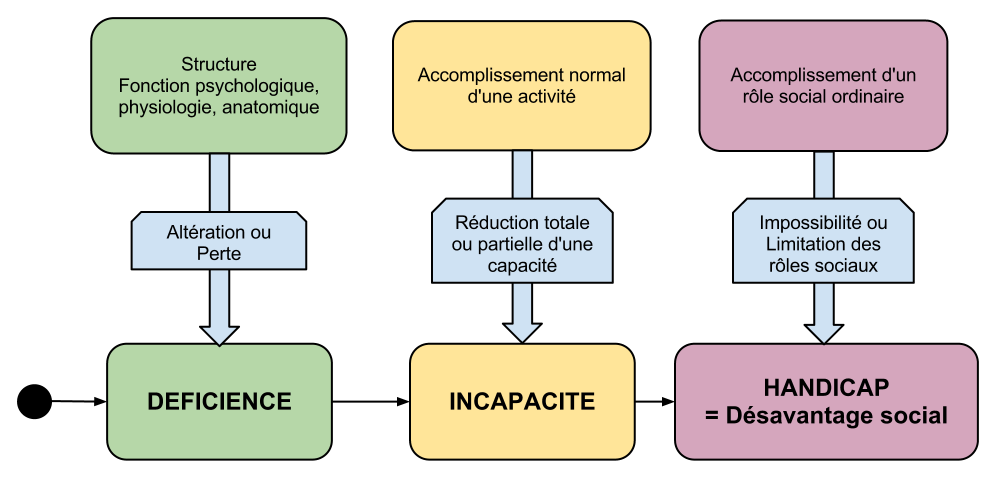
\includegraphics[scale=0.45]{figures/schema_wood.png}
\caption{Définition du Handicap selon le schéma de Wood}
\label{schema_wood}
\end{figure}

C'est pourquoi, pour définir le handicap, il est alors préférable de s'appuyer sur le modèle canadien du "Processus de Production du Handicap" (Figure \ref{modele_canadien}). Ce modèle prend en compte la dimension environnementale d'une personne handicapée (ce que ne faisait pas le schéma de Wood) et sort de la linéarité trop systématique du schéma classique.~\cite{pphFougeyrollas}~\cite{socialConsequences}


\begin{figure}[H]
\centering
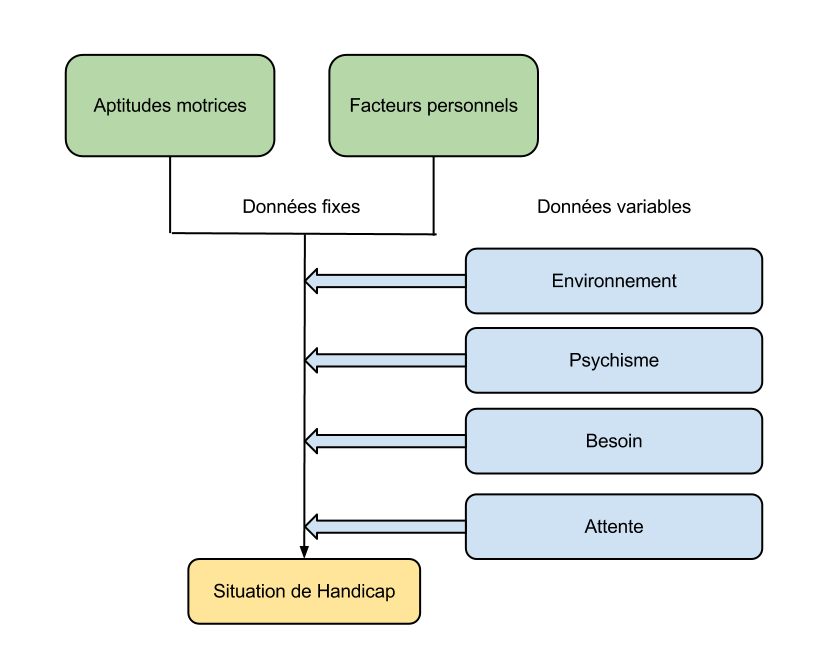
\includegraphics[scale=0.45]{figures/modele_canadien.png}
\caption{Définition du Handicap selon le modèle du canadien Fougeyrollas}
\label{modele_canadien}
\end{figure}

La situation de Handicap devient la résultante de l'interaction entre d'une part l'individu caractérisé par son niveau d'aptitudes motrices et/ou cognitives et ses facteurs personnels (âge, sexe, culture etc.) et l'environnement d'autre part.  \\
Il y a lieu de penser qu'en dehors des facteurs environnementaux, d'autres variables interfèrent avec cette interaction: 
\begin{itemize}
\item Les besoins de la personne handicapée
\item Les attentes de la personne handicapée
\item Le psychisme de la personne\\
\end{itemize}

Toutes ces variables sont par définition labiles.\\


C'est la raison pour laquelle on peut affirmer que le handicap n'est pas un statut mais un \textbf{processus dynamique}, en mouvement permanent. Cette approche nous renvoie en première lecture à notre responsabilité d'agir sur l'environnement pour réduire le handicap. 



\section{Importance des dispositifs législatifs}
Deux lois importantes ont vu le jour au cours de ces 25 dernières années : la loi de 1987 sur l'obligation d'emploi de 6\% de travailleurs handicapées et la loi de 2005.\\

La loi du 10 juillet 1987 oblige les entreprises de 20 salariés et plus à employer 6 \% de personnes handicapées au sein de leurs équipes. Cette loi a permis la création de l'AGEFIPH (Association de Gestion du Fonds pour l'Insertion Professionnelle des Personnes Handicapées) qui récolte des pénalités appelées "contributions", versées par les entreprises ne respectant pas ce quota.\\

La loi du 11 février 2005 augmente la contribution versée en cas de non-respect du quota. Elle renforce également l'égalité des personnes handicapées sur le monde du travail : adaptation technique de poste, formation, accompagnement et aménagement des horaires.\\

Pour une entreprise, lorsque le quota n'est pas respecté, plusieurs cas de figures se présentent :
\begin{itemize}
\item Si l'entreprise possède de 20 à 199 salariés : elle doit alors verser une contribution de 400x le SMIC horaire par bénéficiaire manquant.
\item Si l'entreprise possède plus de 750 salariés : elle doit reverser une contribution de 600x le SMIC horaire par bénéficiaire manquant.
\item Si aucune action n'a été entreprise par l'entreprise dans un délai de 3 ans et qu'aucun salarié n'est un travailleur handicapé, alors l'entreprise doit reverser une contribution de 1500x le SMIC horaire par bénéficiaire manquant (quelque soit la taille de l'entreprise).\\
\end{itemize}

Ce dernier type d'entreprise est appelé "EQZ" ou "Établissements à Quota Zéro". Ces entreprises ne réalisent aucune action en faveur de l'emploi de personnes handicapées. En septembre 2011, 8654 entreprises à Quota Zéro en France ont été dénombrées, ce qui représenterait une proportion de 19\% au niveau national.

\section{Contexte et Problématique}
C'est en prenant la mesure du nombre important d'entreprises à quota zéro et  des entreprises employant moins de 6 \% de personnes handicapées que j'ai pensé mener ma réflexion sur les facteurs explicatifs de cet état de fait et inscrire mon Projet Personnel des Humanités. \\

Durant cette 4e année à l'INSA, j'ai décidé de faire partie de l'association HandiManagement dont le but est de sensibiliser les étudiants sur le campus de l'INSA à l'insertion professionnelle des personnes handicapées et plus généralement au handicap. Les activités de cette association pendant l'année sont séparées en deux phases :
\begin{enumerate}
\item La première phase est appelée l'\textbf{acculturation}. C'est une phase où il nous est proposé de rencontrer des personnes issues du milieu du handicap (associations, personnes effectivement en situation de handicap, responsable de mission au sein des entreprises, etc.). La mission de cette phase est de nous apporter les connaissances nécessaires à la compréhension du dispositifs pour les personnes handicapées en France et de nous mettre en situation directe avec des personnes handicapées pour effacer tout préjugé.
\item La deuxième phase consiste en la préparation d'une semaine de sensibilisation courant mars pour les étudiants de l'INSA où notre r\^ole est de restituer la connaissance acquise, à travers des activités (quizz, pièce de thé\^atre, études de cas managériales, handisport, etc.)\\
\end{enumerate}

Durant la première phase, nous avons eu l'opportunité de rencontrer des entreprises employant plus de 6 \% de personnes handicapées. Ces entreprises avaient développé des missions handicap conséquentes pour permettre une bonne intégration et ainsi pour remplir le quota demandé par l'Agefiph.\\

Cependant, en 2012, près de 49 \% des entreprises \footnote{\url{http://www.agefiph.fr/Entreprises/Contribution-et-obligations/Comment-satisfaire-a-vos-obligations}} ne remplissaient toujours pas le quota demandé par l'Agefiph.\\

A travers ce PPH, je souhaite m'intéresser aux raisons de cette difficulté à embaucher des personnes handicapées.

Mes problématiques sont donc les suivantes :
\begin{itemize}
\item Quels sont, en 2012, les facteurs et les déterminants de la résistance d'une entreprise sur deux à ne pas remplir ses obligations d'emploi de 6 \% des personnes handicapées en référence à la loi de février 2005 sur l'emploi ? \\
\item Quelles pourraient être les réponses concrètes à ce constat ? 
\end{itemize}

